\subsubsection*{Design}
As seen in \cref{img:coredes} the core will consist of a block of memory, an ALU combined with the blitter, and several smaller single function cores.
\begin{figure}[H]
	\centering
	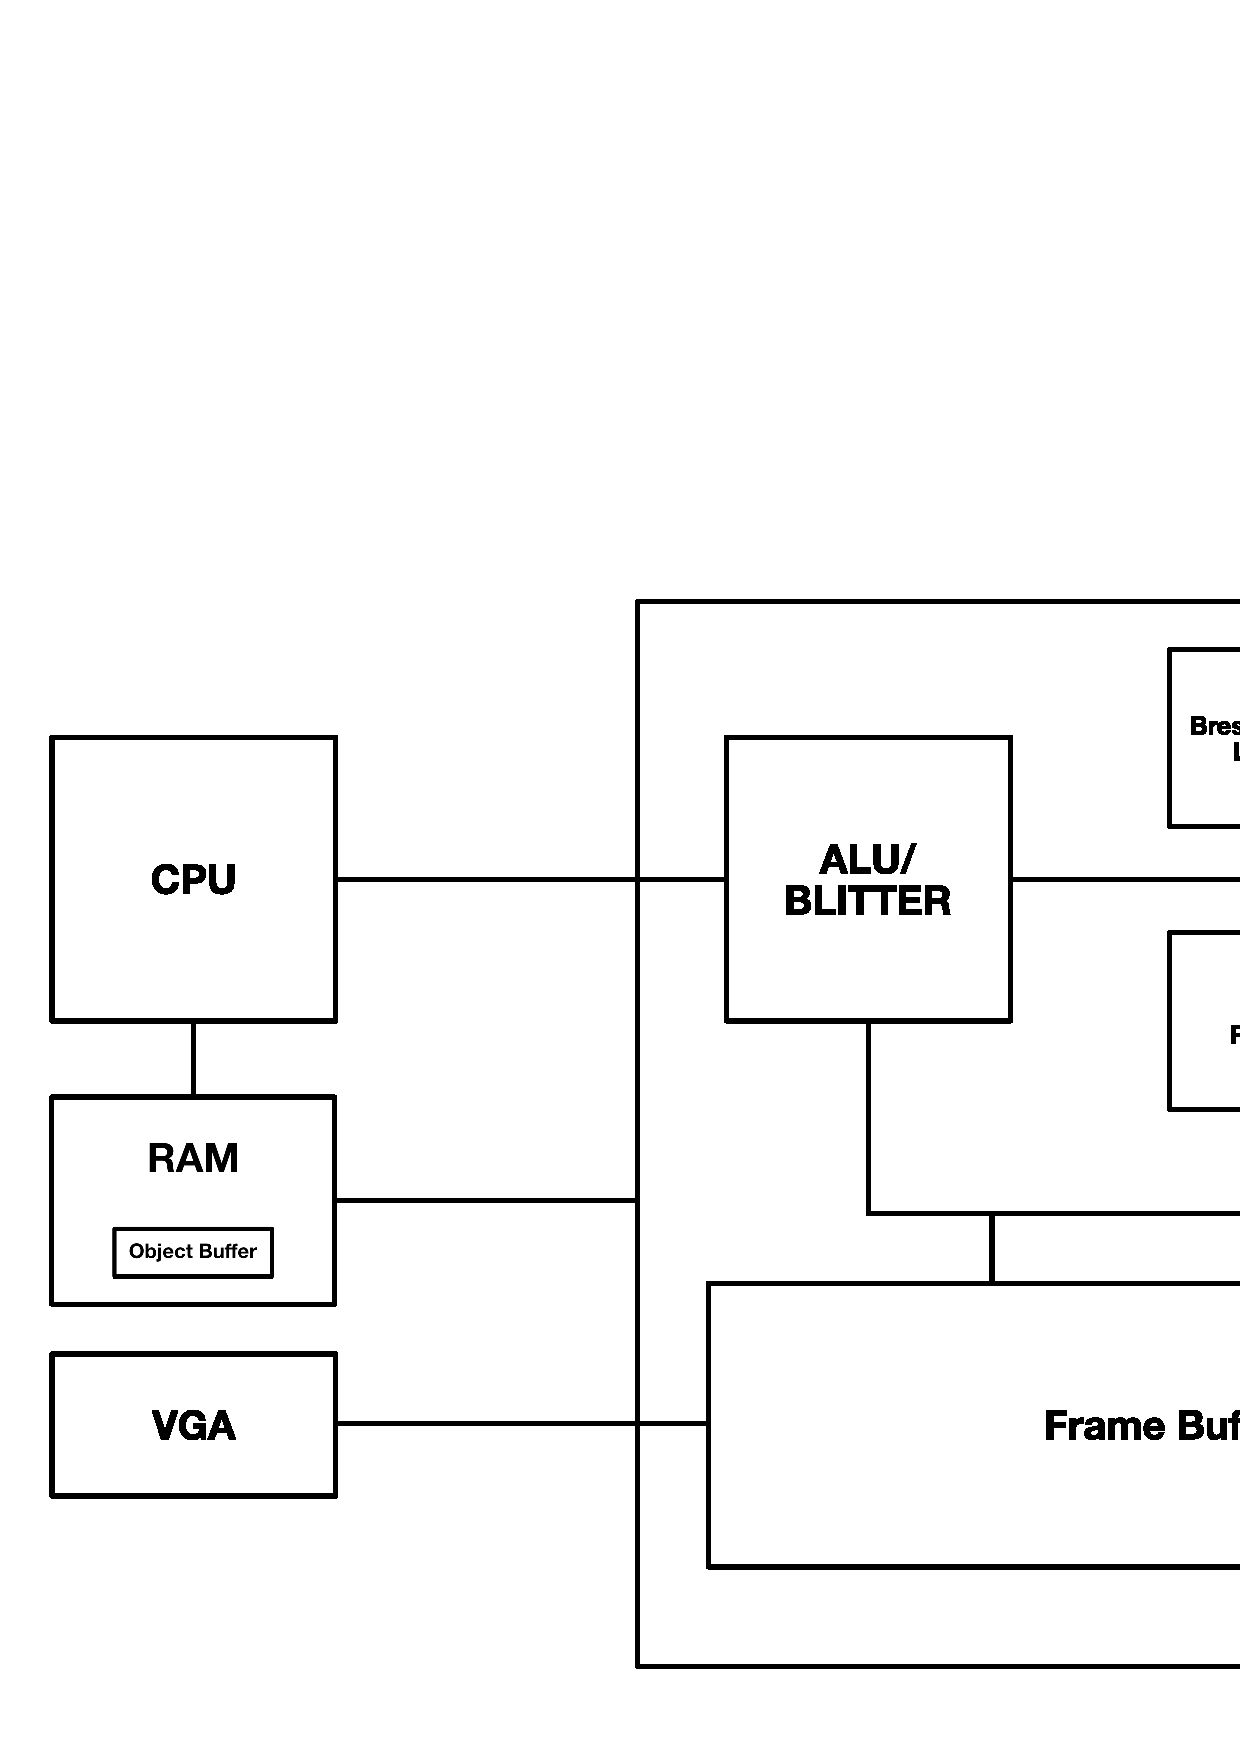
\includegraphics[width=0.5\textwidth]{coredesign}
	\caption{Graphical Design of the AEGIS Core }
	\label{img:coredes}
\end{figure}

The graphic accelerator has a double frame buffer. It keeps track of the information of two separate frames. One of the frames is drawn by the VGA module, the other is being created by the graphics accelerator and CPU. The data for the objects are moved into the RAM of the CPU.

As some functions of the blitter correlate with the functions of the ALU (REFERENCE TO AMIGA MANUAL), the two blocks will be merged together in the following the two of them will be referred to as only the ALU. This part of the core will either write directly into the frame buffer or it will delegate the drawing to the proper function core. These smaller function cores consist of the basic graphical primitives, as discussed in \cref{subsec:des_bresenham}.

For the communication between the CPU and the graphics accelerator, we use two Axi4 buses. The first one is a Axi4Shared for the communication with the CPU, and the second one is a Axi4readonly for the communication with the RAM.

When a write command is send over the AXI4 bus the graphics accelerator looks at the address. Is the address in the range of the double frame buffer, then it writes to it. Otherwise the address determinds, what the graphics accelerator do. Further information he needs to operate get it from RAM at the address in the data value. 

\subsubsection*{Implementation}